\documentclass[a4paper,12pt]{article}

\usepackage[czech]{babel}
\usepackage[utf8]{inputenc}
\usepackage{indentfirst}
\usepackage{hyperref}
\usepackage{graphicx}

\newcommand{\priloha}[1]{\section*{#1}\addcontentsline{toc}{section}{#1}}

\title{Uživatelská dokumentace programu Damebot}
\author{Václav Stupka}
\date{25. května 2025}

\begin{document}
	\maketitle
	\tableofcontents
	
	\section{Úvod}
	Damebot je program, díky kterému si můžete zahrát dámu proti počítači. Tento projekt vznikl jako zápočtový program
	pro předměty Programování v~jazyce C\# a Pokročilé programování v~jazyce C\# na Matematicko-fyzikální fakultě Univerzity
	Karlovy (obor Informatika). 
	
	Tento dokument slouží především jako uživatelská dokumentace. Naleznete zde postup instalace programu, způsob spuštění,
	ovládání a pro při\-po\-me\-nu\-tí také pravidla dámy (ačkoli jsem se snažil respektovat pravidla české dámy, je možné, že se
	mi to ne vždy podařilo).
	
	\section{Instalace a spuštění}
	Program Damebot pro svůj běh vyžaduje framework .NET Desktop verze 8. Tento framework je dostupný pouze na Windows, program Damebot proto nelze spustit na jiných operačních systémech.
	
	Program Damebot je možné stáhnout na adrese
	\url{https://github.com/basvas-jkj/dame_bot/releases/tag/damebot_release}.
	Zde stáhněte soubor \texttt{damebot.zip}
	a extrahujte jeho obsah. Tím je instalace dokončena.
	
	Pro spuštění programu otevřete rozbalenou složku \textit{damebot} a klikněte na soubor \textit{damebot.exe}.
	Tím se hra spustí v~novém okně.
	
	\section{Ovládání}
	V~pravé části obrazovky lze nastavit hru dvou hráčů proti sobě, hru za bílé proti počítači nebo hru za černé proti počítači.
	
	
	\begin{figure}[h]
		\centering
		\includegraphics{img/nastavení}
		\caption{Nastavení hry}
	\end{figure}
	
	
	Pokud není na tahu počítač, je možné začít vlastní tah kliknutím na libovolný kámen hráče, který je právě na tahu.
	Pole pod tímto kamenem zčervená. Následně klikněte na prázdné pole, na které chcete označený kámen přemístit. Pokud je tento tah v~souladu s~pravidly, kámen se přemístí na zvolené pole a odznačí se. Dále je na tahu protivník (podle nastavení druhý hráč nebo počítač).
	
	V~případě, že jste označili některý ze svých kamenů, ale následně jste klikli na pole, na které tento kámen podle pravidel táhnout nemůže, kámen se odznačí a vy můžete vybrat jiný kámen.  Označený kámen se odznačí také v~případě, že myší opustíte plochu šachovnice.
	V~případě vícenásobného skoku je kromě vlastního kamene označeno také každé pole, přes které skok prochází, a to až do chvíle dokončení skoku.
	
	Damebot neprovede svůj tah okamžitě. Nejprve chvíli počká, poté označí modře pole, na kterém stojí kámen, kterým hodlá
	táhnout. Modře se označí také pole, na které příslušný kámen chystá přemístit (v~případě vícenásobného skoku se
	zvýrazní všechna pole, přes která kámen přejde). Následně se příslušný kámen sám přesune. Díky tomu máte možnost lépe sledovat, který kámen se přesunul a na které pole.
	
	V~případě výhry jednoho z~hráčů se nad šachovnicí objeví message box, který nabízí zahajení nové hry (možnost \textit{Ano}),  úplné ukončení programu (možnost \textit{Ne}) nebo zavření boxu nez jakékoli akce (možnost \textit{Zrušit}). Remízu program žádným způsobem nesleduje (není omezený ani počet tahů -- partie může být teoreticky nekonečná).
	
	Novou hru se stejným nastavením lze kdykoli (v~průběhu partie i po jejím skončení) lze zahájit kliknutím na tlačítko \textit{Nová hra}. Novou hru lze spustit také změnou nastavení. V~obou případech se pro potvrzení zobrazí message box.
	
	\section{Pro pokročilé}
	Pokročilí uživatelé mohou mít zájem se podívat také na zdrojový kód programu, případně si vytvořit vlastní modifikaci.
	Patříte-li mezi ně, navštivte webovou stránku projektu \url{https://github.com/basvas-jkj/dame_bot}.
	
	\priloha{Příloha 1 -- pravidla dámy}
	Dáma se hraje na šachovnici (velikost 8×8 polí) se sadou 12~bílých a 12~černých kamenů. Kameny jsou na začátku hry
	rozmístěny v~prvních třech řadách na černých polích (o přípravu hry se stará Damebot). Hru začíná bílý. Kameny se
	pohybují o jedno pole úhlopříčně směrem vpřed (v~tomto případě bílé kameny nahoru a černé dolů). Jestliže je toto
	pole obsazené protivníkovým kamenem a další pole ve stejném směru je volné, může na toto pole posunout svůj kámen.
	Přeskočený kámen je tímto vyhozen a odebrán ze šachovnice. Takový skok je možné provést vícekrát (lze tedy vyhodit
	několik soupeřových kamenů najednou), vždy však musí skákat tentýž kámen (v~jednom tahu nelze provést více skoků
	různými kameny).
	
	Pokud má hráč možnost vyhodit libovolný soupeřův~kámen, je povinen tak učinit. Má-li možnost skákat více kameny,
	může si vybrat kterýkoli z~nich (právě jeden). Rovněž si hráč může vybrat, které kameny přeskočí. Jestliže se hráč
	rozhodne pro vícenásobný skok, musí jej hráč provést celý (skok tedy musí skončit pozicí, ve které skákající kámen
	nemůže vyhodit žádný další protivníkův~kámen).
	
	Kámen, který se dostane na opačný okraj šachovnice, se promění v~dámu. Dáma se může pohybovat úhlopříčně všemi čtyřmi
	směry o libovolný počet polí. Skákat může dáma i přes kameny, které s~ní přímo nesousedí, a skok může ukončit na
	libovolném poli za přeskočeným kamenem (na stejné diagonále). Pokud z~tohoto pole může dále skákat, je povinna tak
	učinit. Při tom může změnit směr. Přes jeden kámen opačné barvy nesmí dáma skočit vícekrát. Toto se nevztahuje na prázdná
	pole (je tedy možné např. začít a skončit tah na stejném poli).
	
	Přes kámen stejné barvy není povoleno skákat (platí pro obyčejné kameny i pro dámu). Pokud se běžný kámen dostane
	na poslední řadu skokem, promění se v~dámu a tah \textbf{končí} (i v~případě, že by proměněná dáma mohla pokračovat
	ve skoku).
	
	Hra končí ve chvíli, kdy jeden z~hráčů přijde o všechny svoje kameny nebo nemůže zahrát další tah (všechny jeho kameny
	jsou zablokované). Vítězem je pak jeho protivník. Remíza by nastala v~případě, kdy při bezchybné hře není ani jeden
	z~hráčů schopen vyhodit nebo zablokovat všechny soupeřovy kameny (např. pokud oběma hráčům zbyde jedna dáma).
	Damebot však tuto možnost nesleduje, hráč se tedy musí sám rozhodnout, zda má smysl v~partii pokračovat.
	
	Na závěr ještě poznamenám, že tato pravidla platí i pro fyzického hráče, i pro Damebota.
	
	\priloha{Příloha 2 -- ukázka programu}
	\begin{figure}[h]
		\centering
		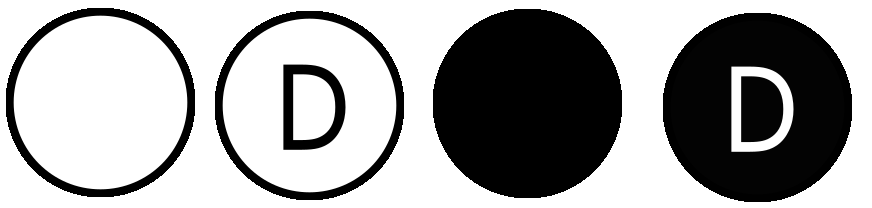
\includegraphics{img/kameny}
		\caption{Zleva bílý kámen, bílá dáma, černý kámen, černá dáma}
	\end{figure}

	\begin{figure}[h]
		\centering
		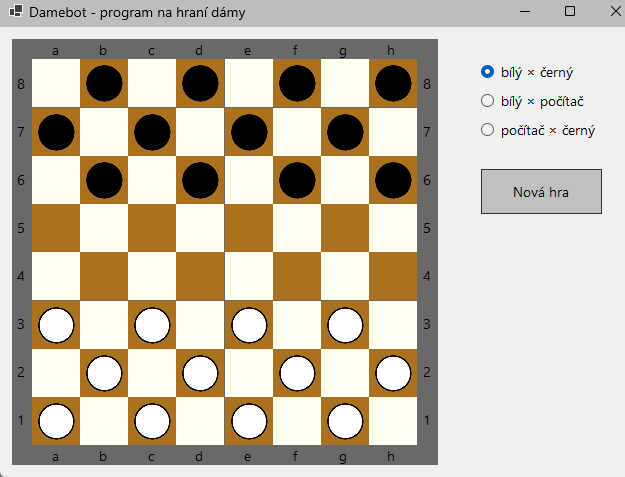
\includegraphics{img/uživatelské_rozhraní}
		\caption{Výchozí pozice}
	\end{figure}

	\begin{figure}[h]
		\centering
		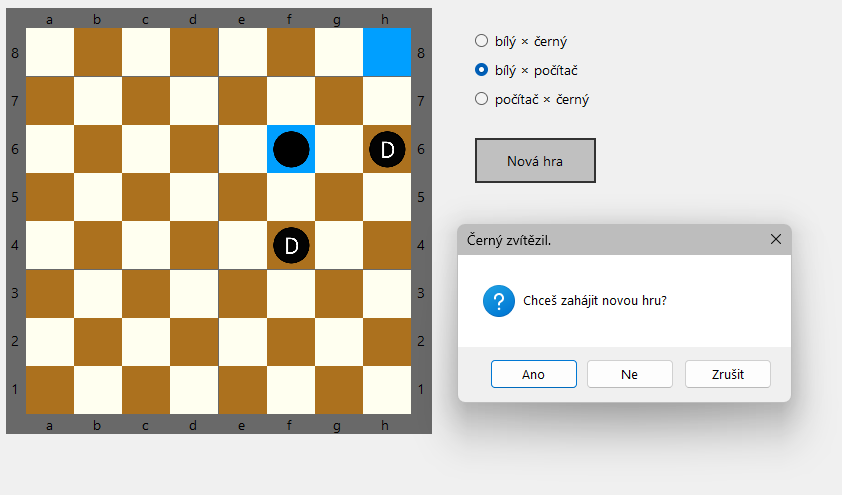
\includegraphics[width=\linewidth]{img/konec_hry}
		\caption{Pozice, ve které černý (Damebot) zvítězil.}
	\end{figure}

	\begin{figure}[h]
		\centering
		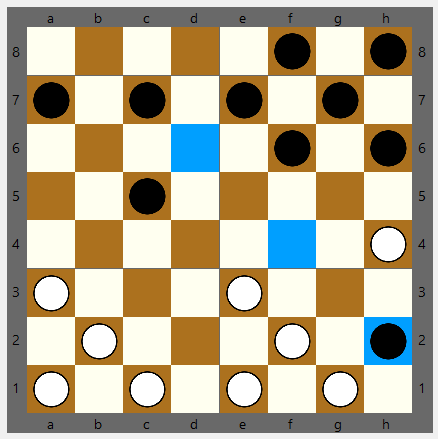
\includegraphics{img/dvojnásobný_skok}
		\caption{Damebot provedl dvojnásobný skok.}
	\end{figure}
\end{document}